\section{Solver Architecture}

The solver is a scientific workflow rather than a general multiphysics model. For each prescribed rounded-cone geometry, it constructs an axisymmetric grid, represents the conductor with either staircase or immersed Dirichlet treatment, solves the sparse Laplace or Poisson system, and reconstructs the gas-side field. Interface normals and curvature then give Maxwell and capillary pressures. The analysis reports either an amplitude-projected stress residual or a log--log flank fit of $E_n^2$ against distance from the virtual vertex (Figure~\ref{fig:solver-flowchart}).

\begin{figure}[H]
\centering
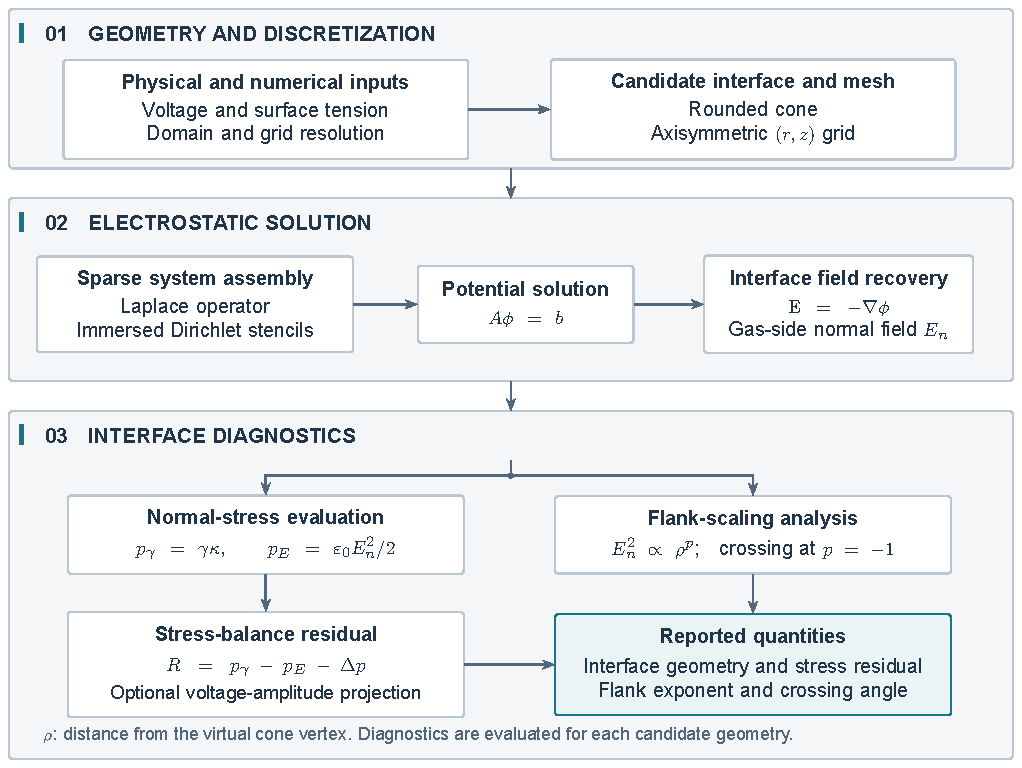
\includegraphics[width=0.98\textwidth]{figures/solver_flowchart_revised.pdf}
\caption{Scientific workflow for the charge-free immersed formulation. A prescribed rounded-cone geometry and boundary condition define the electrostatic solve; interface reconstruction then supplies either the projected stress residual or the flank-field exponent. The exponent crossing is evaluated only where the fitted exponent crosses $-1$.}
\label{fig:solver-flowchart}
\end{figure}

The numerical core uses sparse matrices. Over the measured range of 675--85,073 points, the timing data for a single-threaded immersed Laplace solve follow an empirical $\mathcal{O}(N^{0.99})$ fit; a $121\times177$ grid took approximately $0.46$~s on the machine recorded with the timing data. This fit describes the measured range, not an asymptotic complexity bound.

The associated image workflow renders analytic silhouettes for software tests and extracts contours, centreline registration, flank fits, and profile metrics. Its synthetic tests and its application to published photographs are kept separate: the former tests a known numerical round trip, while the latter provides a secondary-data geometry and stress analysis. Detailed module inventory is omitted from the main text, which is reserved for the numerical method and its verification.
